\documentclass[a4paper]{article}
\usepackage{vntex}
%\usepackage[english,vietnam]{babel}
%\usepackage[utf8]{inputenc}

%\usepackage[utf8]{inputenc}
%\usepackage[francais]{babel}
\usepackage{a4wide,amssymb,epsfig,latexsym,array,hhline,fancyhdr}
\usepackage{booktabs}
\usepackage[table,xcdraw]{xcolor}
\usepackage{amsmath}
\usepackage{amsthm}
\usepackage{multicol,longtable,amscd}
\usepackage{diagbox}%Make diagonal lines in tables
\usepackage{booktabs}
\usepackage{alltt}
\usepackage[framemethod=tikz]{mdframed}% For highlighting paragraph backgrounds
\usepackage{caption,subcaption}

\usepackage{lastpage}
\usepackage[lined,boxed,commentsnumbered]{algorithm2e}
\usepackage{enumerate}
\usepackage{color}
\usepackage{graphicx}							% Standard graphics package
\usepackage{array}
\usepackage{tabularx, caption}
\usepackage{multirow}
\usepackage{multicol}
\usepackage{rotating}
\usepackage{graphics}
\usepackage{geometry}
\usepackage{setspace}
\usepackage{epsfig}
\usepackage{tikz}
\usetikzlibrary{arrows,snakes,backgrounds}
\usepackage[unicode]{hyperref}
\hypersetup{urlcolor=blue,linkcolor=black,citecolor=black,colorlinks=true} 
%\usepackage{pstcol} 								% PSTricks with the standard color package

\newtheorem{theorem}{{\bf Định lý}}
\newtheorem{property}{{\bf Tính chất}}
\newtheorem{proposition}{{\bf Mệnh đề}}
\newtheorem{corollary}[proposition]{{\bf Hệ quả}}
\newtheorem{lemma}[proposition]{{\bf Bổ đề}}


%\usepackage{fancyhdr}
\setlength{\headheight}{40pt}
\pagestyle{fancy}
\fancyhead{} % clear all header fields
\fancyhead[L]{
 \begin{tabular}{rl}
    \begin{picture}(25,15)(0,0)
    \put(0,-8){
\includegraphics[width=8mm, height=8mm]{Images/hcmut.png}}
    %\put(0,-8){\epsfig{width=10mm,figure=hcmut.eps}}
   \end{picture}&
	%
\includegraphics[width=8mm, height=8mm]{hcmut.png} & %
	\begin{tabular}{l}
		\textbf{\bf \ttfamily Trường Đại Học Bách Khoa Tp.Hồ Chí Minh}\\
		\textbf{\bf \ttfamily Khoa Khoa Học và Kỹ Thuật Máy Tính}
	\end{tabular} 	
 \end{tabular}
}
\fancyhead[R]{
	\begin{tabular}{l}
		\tiny \bf \\
		\tiny \bf 
	\end{tabular}  }
\fancyfoot{} % clear all footer fields
\fancyfoot[L]{\scriptsize \ttfamily Bài tập lớn môn Mô hình hóa toán học (CO2011) - Niên khóa 2019-2020}
\fancyfoot[R]{\scriptsize \ttfamily Trang {\thepage}/\pageref{LastPage}}
\renewcommand{\headrulewidth}{0.3pt}
\renewcommand{\footrulewidth}{0.3pt}


%%%
\setcounter{secnumdepth}{4}
\setcounter{tocdepth}{3}
\makeatletter
\newcounter {subsubsubsection}[subsubsection]
\renewcommand\thesubsubsubsection{\thesubsubsection .\@alph\c@subsubsubsection}
\newcommand\subsubsubsection{\@startsection{subsubsubsection}{4}{\z@}%
                                     {-3.25ex\@plus -1ex \@minus -.2ex}%
                                     {1.5ex \@plus .2ex}%
                                     {\normalfont\normalsize\bfseries}}
\newcommand*\l@subsubsubsection{\@dottedtocline{3}{10.0em}{4.1em}}
\newcommand*{\subsubsubsectionmark}[1]{}
\makeatother

\everymath{\color{blue}}%make in-line maths symbols blue to read/check easily

\sloppy
\captionsetup[figure]{labelfont={small,bf},textfont={small,it},belowskip=-1pt,aboveskip=-9pt}
%space remove between caption, figure, and text
\captionsetup[table]{labelfont={small,bf},textfont={small,it},belowskip=-1pt,aboveskip=7pt}
%space remove between caption, table, and text

%\floatplacement{figure}{H}%forced here float placement automatically for figures
%\floatplacement{table}{H}%forced here float placement automatically for table
%the following settings (11 lines) are to remove white space before or after the figures and tables
%\setcounter{topnumber}{2}
%\setcounter{bottomnumber}{2}
%\setcounter{totalnumber}{4}
%\renewcommand{\topfraction}{0.85}
%\renewcommand{\bottomfraction}{0.85}
%\renewcommand{\textfraction}{0.15}
%\renewcommand{\floatpagefraction}{0.8}
%\renewcommand{\textfraction}{0.1}
\setlength{\floatsep}{5pt plus 2pt minus 2pt}
\setlength{\textfloatsep}{5pt plus 2pt minus 2pt}
\setlength{\intextsep}{10pt plus 2pt minus 2pt}

\begin{document}

\begin{titlepage}
\begin{center}
ĐẠI HỌC QUỐC GIA THÀNH PHỐ HỒ CHÍ MINH \\
TRƯỜNG ĐẠI HỌC BÁCH KHOA \\
KHOA KHOA HỌC - KỸ THUẬT MÁY TÍNH 
\end{center}

\vspace{1cm}

\begin{figure}[h!]
\begin{center}

\includegraphics[width=3cm]{Images/hcmut.png}
\end{center}
\end{figure}

\vspace{1cm}


\begin{center}
\begin{tabular}{c}
\multicolumn{1}{l}{\textbf{{\Large MÔ HÌNH HÓA TOÁN HỌC (CO2011)}}}\\
~~\\
\hline
\\
\multicolumn{1}{l}{\textbf{{\Large Nhóm: GoPro ---- Bài tập lớn}}}\\
\\
\textbf{{\Huge Mô hình SIR}} \\
\textbf{{\Huge trong dự báo COVID-19}}\\
\\
\hline
\end{tabular}
\end{center}

\vspace{1.5cm}

\begin{table}[h]
\begin{tabular}{rrl}
\hspace{5 cm} & GVHD: & Nguyễn An Khương\\
\hspace{5 cm} &  & Nguyễn Tiến Thịnh\\

& SV thực hiện: & Sỳ Tùng An -- 1811389 \\
& & Huỳnh Tuấn Anh -- 1811408 \\
& & Vũ Nguyễn Minh Đạt -- 1811904  \\
& & Hồ Văn Lợi -- 1811068\\
& & Hồ Quang Khải -- 1810995 \\
\end{tabular}
\end{table}
\vspace{1.5cm}
\begin{center}
{\footnotesize Tp. Hồ Chí Minh, Tháng 7/2020}
\end{center}
\end{titlepage}


%\thispagestyle{empty}

\newpage
\tableofcontents
\newpage

Bài báo cáo này trình bày lời giải một số bài toán trong bài tập lớn môn học Mô hình hóa Toán học với chủ đề là: Mô hình SIR trong dự báo Covid-19.
%%%%%%%%%%%%%%%%%%%%%%%%%%%%%%%%%
\section{Bài toán 1}
\subsection{Mô hình SIR}
Mô hình SIR (Suspectible - Infectious - Recovered) là một trong các mô hình cách ly cơ bản được sử dụng nhiều nhất trong quá khứ và hiện tại để mô tả dịch bệnh. Mô hình này đươc giới thiệu trong bài báo kinh điển của Kermack và McKendrick vào thế kỷ XX. Trong mô hình này có 3 trạng thái: 
\begin{itemize}
    \item Có nguy cơ mắc bệnh
    \item Mắc bệnh
    \item Hồi phục
\end{itemize}
Trạng thái này có thể chuyển từ có nguy cơ mắc bệnh sang mắc bệnh, hoặc từ mắc bệnh sang hồi phục. Giả thiết rằng sẽ miễn dịch với bệnh nếu đã phục hồi.\\
Mô hình SIR là một hệ động lực gồm ba phương trình vi phân sau:
\\

\begin{align}
    \frac{dS}{dt} = -\frac{\beta}{N}IS,
    \\
    \frac{dI}{dt} = \frac{\beta}{N}IS - \gamma I,
    \\
    \frac{dR}{dt} = \gamma I
\end{align}
Trong đó, tại mỗi thời điểm $t \geq t_{0} \geq 0$ với $t_{0}$ là thời điểm đầu ghi nhận
\begin{itemize}
    \item S(t): Số người có nguy cơ mắc bệnh;
    \item I(t): Số người nhiễm bệnh;
    \item R(t): Số người phục hồi sau bệnh;
    \item $\beta (t)$: Tỷ lệ tiếp xúc của mỗi người trong nhóm S(t) với người trong nhóm I(t);
    \item $\gama(t)$: Tỷ lệ hồi phục khi mắc bệnh;
    \item N(t): Tổng số người trong cộng đồng bị cách ly được tính bằng:
\begin{align}
    N(t) = S(t) + I(t) + R(t)
\end{align}
\end{itemize}
Hệ phương trình vi phân trên có thể hiểu như sau:
\begin{itemize}
    \item Phương trình (1) thể hiện sự suy giảm số người có nguy cơ mắc bênh tại thời điểm t $\geq$ t0. Sự suy giảm được tính theo xác suất lây bệnh khi có tiếp xúc giữa nhóm S(t) và I(t).
    \item Phương trình (2) thể hiện độ biến thiên số người mắc bệnh tại thời điểm t $\geq$ t0. Sự biến thiên này được tính bằng cách lấy số người ở nhóm S(t) đã bị lây nhiễm sau khi tiếp xúc với người bệnh nhóm I(t) và trừ đi số người ở nhóm I(t) đã hồi phục theo tỷ lệ $\gamma I(t)$.
    \item Phương trình (3) thể hiện số người đã hồi phục từ nhóm I(t) theo tỷ lệ hồi phục là $\gamma$.
\end{itemize}
\newpage
Hệ số lây nhiễm cơ bản$ R_{0}$: Là một trong những đại lượng cơ bản quan trọng nhất đối với một mô hình dịch bệnh.
\begin{itemize}
    \item Nếu $R_{0} < 1$ dịch sẽ tắt trước khi bùng phát
    \item $R > 0$ dịch sẽ bùng phát.
\end{itemize}
Ví dụ :
\begin{itemize}
    \item Theo mô hình SIR ở trên, $R_{0} = BN/\gamma$.
Trong đó BN là số người khỏe mạnh trung bình mà môt người mắc bệnh có thể lây cho trong khoảng thời gian mắc bệnh
    \item Mặt khác : nếu trung bình một người mắc bệnh lây cho nhiều hơn một người thì số người mắc bệnh phải tăng theo cấp số nhân, còn nếu một người mắc bệnh lây cho ít hơn một người khác thì số người mắc bệnh phải giảm dần.
\end{itemize}
\textbf{Ví dụ 1.1:} Giả sử có một loại cúm đang lây lan trong một cộng đồng dân cư. Giả sử rằng:
\begin{itemize}
    \item Cộng đồng này đang bị cách ly.
    \item Loại cúm này có thời gian từ khi phát bệnh đến khi hồi phục là 5/3 tuần không đổi theo thời gian.
    \item  Giả thiết rằng người bị nhiễm sẽ miễn dịch với bệnh nếu đã phục hồi.
    \item Tỷ lệ mắc bệnh khi có tiếp xúc với người bệnh ở mức $0,2$ sau một tuần tiếp xúc và tỷ lệ này không đổi theo thời gian.
\end{itemize}
Khi đó, với mỗi tuần, theo mô hình ta có:

\begin{align}
    \frac{dS}{dt} = 0,6I.\\
    \frac{dI}{dt} = 0,001407IS - 0,6I\\
    \frac{dR}{dt} = -0,001407IS
\end{align}







\\
 \begin{figure}[!ht] 
    \label{Fig:Frequency}
	\begin{center}
	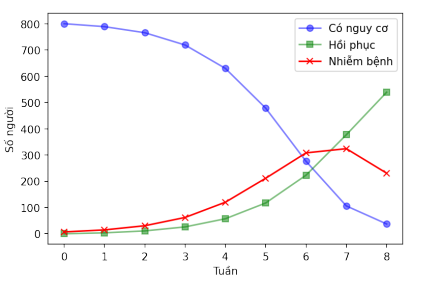
\includegraphics[scale=1.2]{Images/img1.1.png}
	\caption{Số ca mắc bệnh tăng trong khoảng 6 tuần đầu tiên và giảm dần ở 2 tuần tiếp theo }
	\end{center}
\end{figure}

% \begin{center}
%     \begin{figure}[!ht]
%     \begin{center}
%      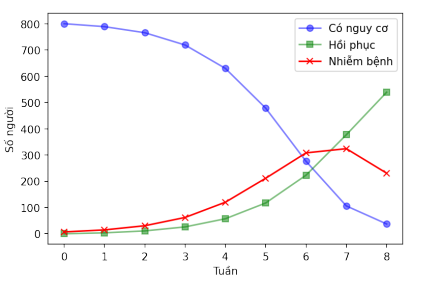
\includegraphics[scale=1.2]{Images/img1.1.png}
%     \end{center}
%     \caption{Số ca mắc bệnh tăng trong khoảng 6 tuần đầu tiên và giảm dần ở 2 tuần tiếp theo}
%     \label{refhinh1}
%     \end{figure}
% \end{center}




\break 

\subsection{Trường hợp rời rạc: Ước lượng hệ số  $\beta$ và $\gamma$}
Phương án cách ly từng nhóm người đã từng tiếp xúc trực tiếp hoặc gián tiếp với người nhiễm bệnh được xem là phương pháp tốt nhất để khống chế dịch bệnh. Tuy nhiên ta xét các hệ số $\beta$ và $\gamma$ có thể biến đổi theo thời gian do có sự điều chỉnh trong lệnh cách ly. Từ đó, cơ hội tiếp xúc với người bệnh giảm hoặc tăng dẫn đến xác suất nhiểm $\beta$ thay đổi. Khi tình trạng các bệnh viện quá tải, sự tập trung của các y bác sĩ cho từng bệnh nhân có sự thay đổi và dẫn đến tỷ lệ hồi phục cũng thay đổi theo thời gian.\\ 
Việc ước lượng các hệ số $\beta$ và $\gamma$ phụ thuộc vào dữ liệu đã công bố. Cụ thể là số ca mắc bệnh và phục hồi tích lũy theo thời gian.

Ở đây ta sẽ sử dụng phương pháp suy luận Bayes, gọi:
\begin{itemize}
    \item $X$: biến ngẫu nhiên quan sát số ca mắc bệnh và số ca hồi phục tại từng thời điểm $t \geq t_{0}$;
    \item $\pi (\beta,\gamma|X)$: phân bố xác suất hậu nghiệm của  $\beta$ và $\gamma$  khi có dữ liệu quan sát;
    \item $\pi (X|\beta,\gamma)$: phân bố xác suất của số ca mắc bệnh và số ca phục hồi;
    \item$\pi (\beta,\gamma)$: phân bố xác suất tiên nghiệm khi chưa có dữ liệu ghi nhận về số ca mắc bệnh và số ca phục hồi.
\end{itemize}
Định lý Bayes:
\begin{align}
    \pi (\beta,\gamma|X) \propto \pi (X|\beta,\gamma \pi (\beta,\gamma)
\end{align}
Phân bố các suất hậu nghiệm của $\beta$ và $\gamma$ có thể được tính bằng cách lấy phân bố xác suất của số ca mắc bệnh và số ca phục hồi  khi $\beta$ và $\gamma$ cho trước nhân với phân bố xác suất tiên nghiệm của $\beta$ và $\gamma$.

\subsection{Trường hợp liên tục: Phương pháp xấp xỉ Euler}
Trong toán học và khoa học máy tính, phương pháp Euler là một phương pháp số bậc một để giải các phương trình vi phân thường với giá trị ban đầu cho trước\\
Giả sử ta có phương trình vi phân bậc nhất:
\begin{align}
    y' = f(t,y(t)).
\end{align}
Ý tưởng của phương pháp Euler là xấp xỉ nghiệm $y$ bằng dãy ${y_{n}}$ sao cho:
\begin{align}
    y_{n+1} = y_{n} + f(t_{n},y_{n}) \Delta{t}
\end{align}
Với $\Delta{t}$ là bước xấp xỉ đủ nhỏ và $f(t_{n},y_{n})$ là độ dốc của đường cong $y$ tính tại thời điểm $t$
Tổng quát, hệ phương trình vi phân bậc 1 được viết dưới dạng
\begin{align}
    y'_{1} = f_{1}(t,y_{1},...,y_{N}),
\end{align}
\centerline{\vdots}
\begin{align}
    y'_{N} = f_{N}(t,y_{1},...,y_{N}),
\end{align}
Trong đó $y_{i}$ là các hàm số thực phụ thuộc vào biến  $t \geq t_{0}$ và $f_{i}$ là các hàm số thực phi tuyến phụ thuộc vào biến  $t \geq t_{0}$ và cac $y'_{i}$ với mọi $i \in {1,...,N}$. Phương pháp Euler khi đó được áp dụng cho từng $y_{i}$.
\begin{center}
    \begin{figure}[htp]
    \begin{center}
     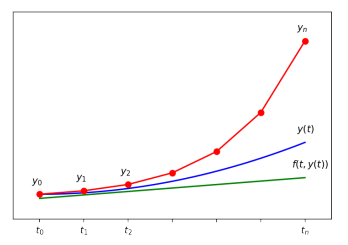
\includegraphics[scale=1.3]{Images/img1.2.PNG}
    \end{center}
    \caption{Các điểm tròn màu đỏ chính là giá trị xấp xỉ đường cong $y$ có độ dốc $f(t,y)$}
    \label{refhinh2}
    \end{figure}
\end{center}
\subsection{Mô hình SIRD}
Mô hình SIRD (Susceptible-Infectious-Recovered-Deceased) phân biệt giữa hồi phục (Recovered - sống sót sau khi mắc bệnh và đã được miễn dịch) với đã chết (Deceased). Mô hình SIRD gồm các phương trình vi phân sau: 
\begin{align}
    \frac{dS}{dt} = -\frac{\beta}{N}IS,
    \\
    \frac{dI}{dt} = \frac{\beta}{N}IS - \gamma I - \varphi I,
    \\
    \frac{dR}{dt} = \gamma I,
    \\
    \frac{dD}{dt} = \varphi I
\end{align}
Với các đại lượng tương tự như mô hình SIR, ngoài ra:
\begin{itemize}
    \item $D(t)$: Số người tử vong;
    \item $\varphi(t)$: Tỷ lệ tử vong.
\end{itemize}
Hệ phương trình vi phân trên có thể hiểu như sau:
\begin{itemize}
    \item Phương trình (1) thể hiện sự suy giảm số người có nguy cơ mắc bênh tại thời điểm t $\geq$ t0. Sự suy giảm được tính theo xác suất lây bệnh khi có tiếp xúc giữa nhóm S(t) và I(t).
    \item Phương trình (2) thể hiện độ biến thiên số người mắc bệnh tại thời điểm t $\geq$ t0. Sự biến thiên này được tính bằng cách lấy số người ở nhóm S(t) đã bị lây nhiễm sau khi tiếp xúc với người bệnh nhóm I(t) trừ đi tổng của số người ở nhóm I(t) đã hồi phục theo tỷ lệ $\gamma I(t)$ và đã tử vong theo tỷ lệ $\varphi I(t)$.
    \item Phương trình (3) thể hiện số người đã hồi phục từ nhóm I(t) theo tỷ lệ hồi phục là $\gamma$.
    \item Phương trình (4) thể hiện số người đã tử vong từ nhóm I(t) theo tỷ lệ tử vong là $\varphi$.
\end{itemize}
\textbf{Ví dụ 1.2:} Có một loại cúm đang lây lan trong cộng đồng dân cư, giả sử rằng:
\begin{itemize}
    \item Cộng đồng này đang bị cách ly.
    \item  Giả thiết rằng người bị nhiễm sẽ miễn dịch với bệnh nếu đã phục hồi.
    \item $S(0) = 997, I(0) = 3, R(0) = 0$ và các tỷ lệ $\beta = 0.4, \gamma = 0.035, \varphi = 0.005$
\end{itemize}
Ta có biểu đồ sau: 
\begin{center}
    \begin{figure}[htp]
    \begin{center}
     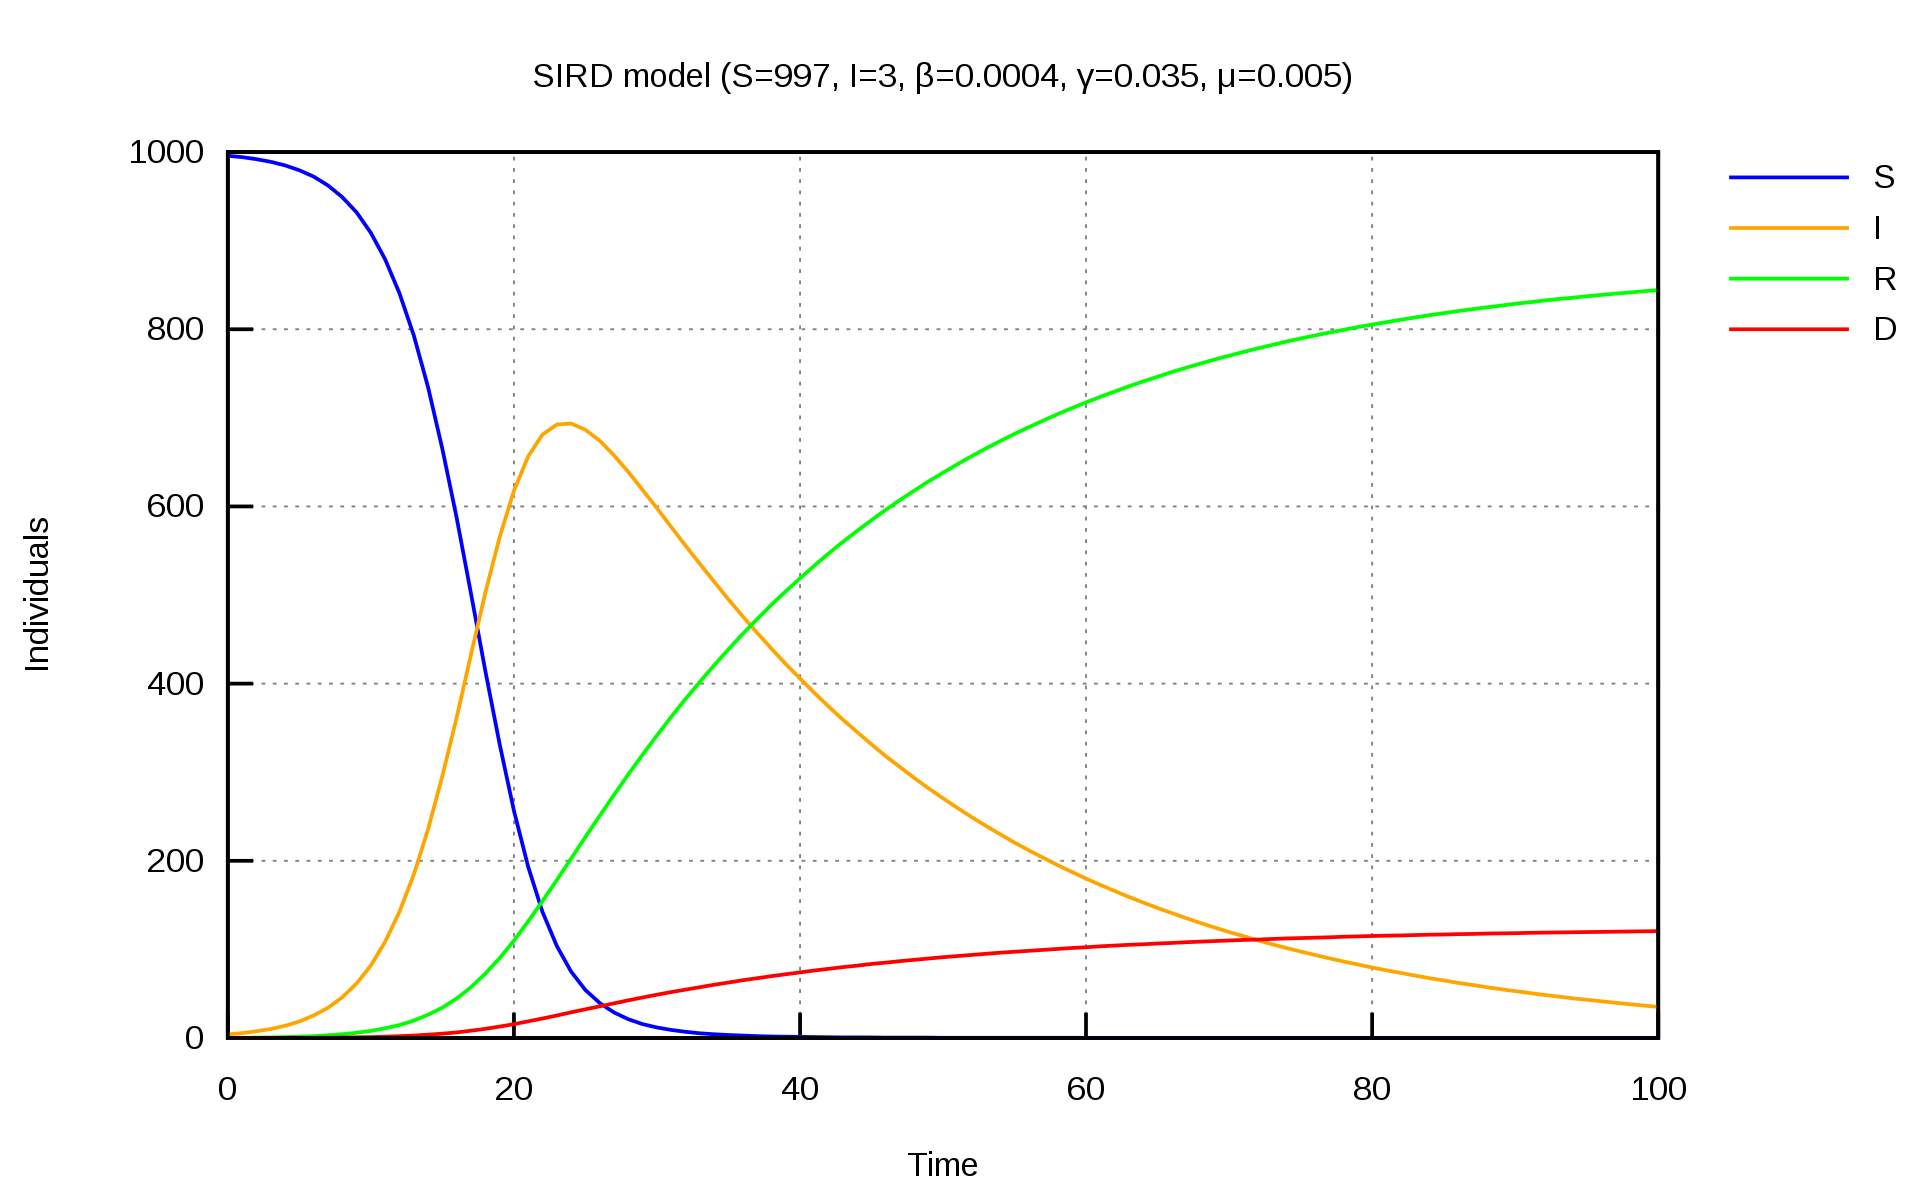
\includegraphics[scale=.15]{Images/img1.3.PNG}
    \end{center}
    \caption{Biểu đồ mô hình SIRD với các giá trị ban đầu và tỷ lệ nhiễm trùng, phục hồi và tử vong}
    \label{refhinh3}
    \end{figure}
\end{center}

%%%%%%%%%%%%%%%%%%%%%%%%%%%%%%%%%
\newpage
\section{Bài toán 2}
\subsection{Thiết lập chương trình}
Để giải quyết bài toán, chúng em đã hiện thực một chương trình với ngôn ngữ Python 3.8.3 32-bit, đầu tiên chúng em sử dụng các thư viên của python như {\tt numpy} (hỗ trợ tính toán),  {\tt odeint} (hỗ trợ tính vi phân), và {\tt matplotlib.pyplot} (hỗ trợ vẽ đồ thị).

\begin{mdframed}[hidealllines=true,backgroundcolor=magenta!10]
\begin{alltt}
\textit{
import numpy as np
from scipy.integrate import odeint
import matplotlib.pyplot as plt
}
\end{alltt}
\end{mdframed}

Ta xây dựng mô hình SIR dựa thể hiện ba trạng thái (Có nguy cơ mắc bệnh - Mắc bệnh - Hồi phục) cho nhóm người được cách ly với giả thuyết rằng sẽ có miễn dịch với bệnh nếu đã phục hồi. Và đối với trường hợp khác của nó là mô hình SIRD thể hiện 4 trạng thái (Có nguy cơ mắc bệnh - Mắc bệnh - Hồi phục - Tử vong) dựa trên cơ sở lí thuyết đã trình bày trong bài toán số 1

Mô hình SIR được hiện thực với python như sau:


\begin{mdframed}[hidealllines=true,backgroundcolor=magenta!10]
\begin{alltt}
\textit{
def SIR(y, t, N, beta, gamma):
    S, I, R = y
    dS_dt = -(beta/N) * I * S
    dI_dt = (beta/N) * I * S - gamma * I
    dR_dt = gamma * I
    # return dS_dt, dI_dt, dR_dt
    return dS_dt, dI_dt, dR_dt

}
\end{alltt}
\end{mdframed}

Mô hình SIRD được hiện thực với python như sau:

\begin{mdframed}[hidealllines=true,backgroundcolor=magenta!10]
\begin{alltt}
\textit{
def SIRD(y, t, N, beta, gamma):
    S, I, R, D = y
    dS_dt = -(beta/N) * I * S
    dI_dt = (beta/N) * I * S - (gamma * I)/(1-ro)
    dR_dt = gamma * I
    dD_dt = (ro * gamma * I)/(1-ro)
    # return dS_dt, dI_dt, dR_dt
    return dS_dt, dI_dt, dR_dt, dD_dt

}
\end{alltt}
\end{mdframed}

Dùng {\tt odeint} để tính toán với công thức Euler trong mô hình SIR:
\begin{mdframed}[hidealllines=true,backgroundcolor=magenta!10]
\begin{alltt}
\textit{
 y0 = S0, I0, R0
    result = odeint(SIR, y0, t, args=(N, beta, gamma))
    S, I, R = result.T
}
\end{alltt}
\end{mdframed}

Tương tự với mô hình SIRD:

\begin{mdframed}[hidealllines=true,backgroundcolor=magenta!10]
\begin{alltt}
\textit{
 y0 = S0, I0, R0, D0
    result = odeint(SIRD, y0, t, args=(N, beta, gamma))
    S, I, R, D = result.T
}
\end{alltt}
\end{mdframed}

\subsection{Hiện thực hóa chương trình}
Giả sử tại thời điểm ban đầu:
\begin{itemize}
    \item Số người trong cộng đồng là 1000 người, số người mắc bệnh là 2  người, số ca hồi phục và tử vong khi ấy chưa có.
    \item Tỷ lệ người có nguy cơ mắc bệnh tiếp xúc với người nhiễm bệnh là  $\beta = 20\%$
    \item Tỷ lệ người hồi phục sau khi mắc bệnh là  $\gamma = 10\%$
    \item Tỷ lệ tử vong là  $\varphi = 1\%$
    
\end{itemize}
Sử dụng phương pháp Euler, ta sẽ giải hệ SIR và SIRD để tìm ra số người có khả năng bị lấy nhiễm, số người mắc bệnh, số ca hồi phục và số ca tử vong sau 200 ngày tính từ thời điểm đầu ghi nhận số liệu.

\\\\
Khi khởi chạy chương trình,trong trường hợp hệ {\tt SIR} điều kiện ban đầu là:


\begin{mdframed}[hidealllines=true,backgroundcolor=blue!10]
\begin{alltt}
\textit{
# after this trail is a comment
SIR or SIRD? Press 1 to choose SIR, otherwise press 2
1
Number of individuals: 1000
Time: 200  
Beta: 0.2 
Gamma: 0.1
Initial number of Infected: 2
Initial number of Recovered: 0
}
\end{alltt}
\end{mdframed}

Ta thu được biểu đồ:

\begin{figure}[!ht]\caption{Đồ thị thể hiện  ${I(t)}$, ${R(t)}$ và ${D(t)}$ tại thời điểm ${t  \geq  t_{0}}$ } \label{Fig:Frequency}
	\begin{center}
	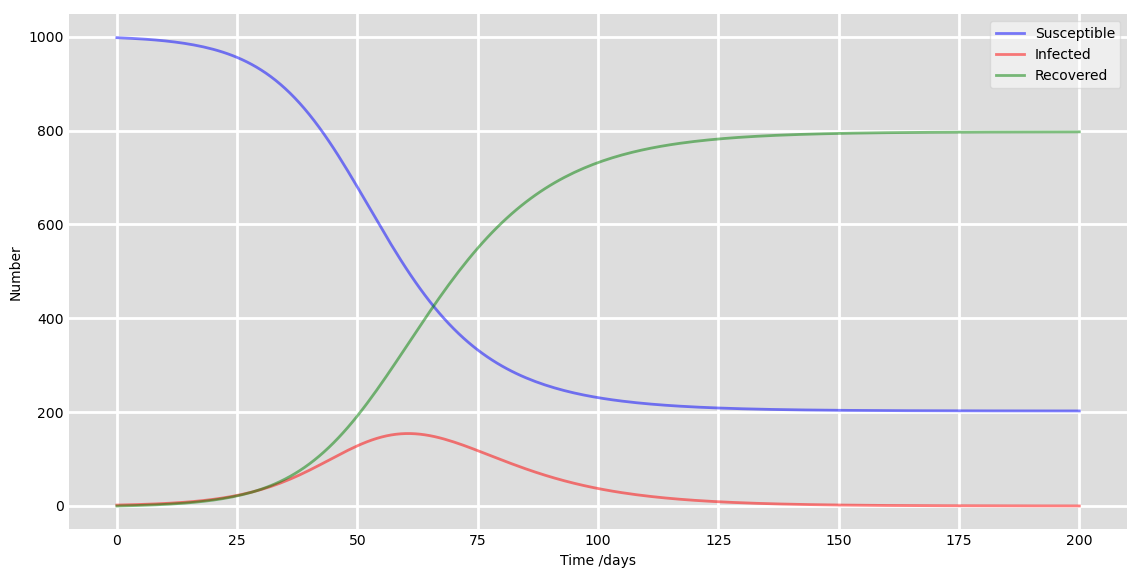
\includegraphics[scale=0.5]{Images/Frequency.png}
	\end{center}
\end{figure}
\break 
Đối với trường hợp hệ {\tt SIRD}:

\begin{mdframed}[hidealllines=true,backgroundcolor=blue!10]
\begin{alltt}
\textit{
SIR or SIRD? Press 1 to choose SIR, otherwise press 2
2
Number of individuals: 1000
Time: 200
Beta: 0.2
Gamma: 0.1
Phi: 0.01
Initial number of Infected: 2
Initial number of Recovered: 0
Initial number of Deceased: 0
}
\end{alltt}
\end{mdframed}

Ta thu được biểu đồ như sau:

\begin{figure}[!ht]\caption{ Đồ thị thể hiện  ${I(t)}$, ${R(t)}$ và ${D(t)}$ tại thời điểm t  $\geq$  $t_{0}$ }  \label{Fig:Frequency1}
	\begin{center}
	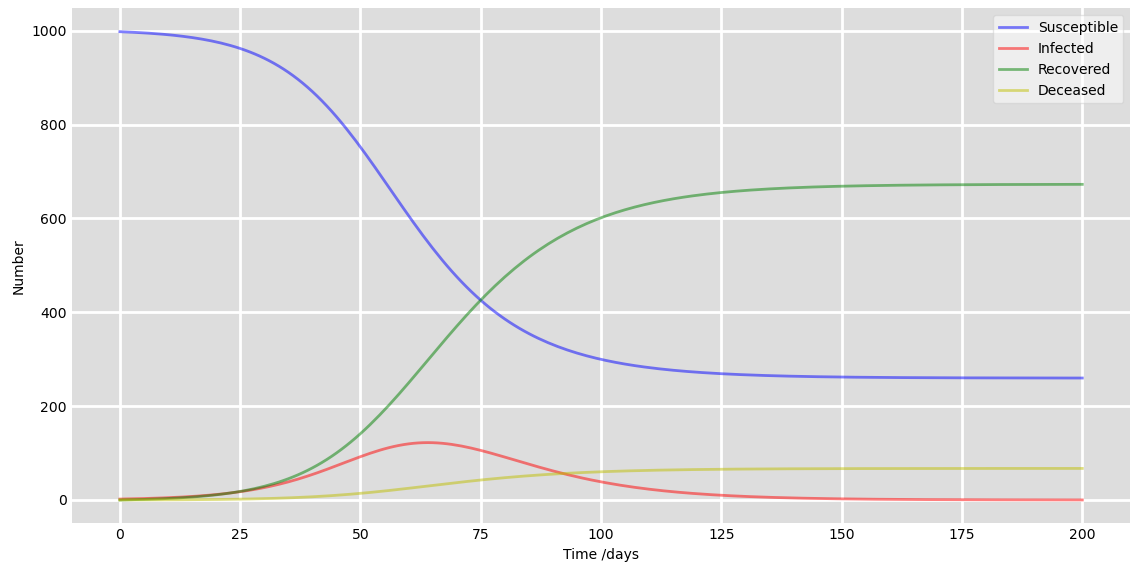
\includegraphics[scale=0.5]{Images/Frequency2.png}
	\end{center}
\end{figure}

\break 
%%%%%%%%%%%%%%%%%%%%%%%%%%%%%%%%%
\newpage
\section{Bài toán 3}
\subsection{Thiết lập chương trình}
Để ướng lượng được hệ số của $\beta$ và $\gamma$ ta sử dụng các bước của thuật toán Metropolis–Hastings:
	 \begin{enumerate}
	 \item Biến $\beta_{0}$ và $\gamma_{0}$ được chọn từ xác xuất tiên nghiệm ở đây sử dụng hàm gammar.pdf với tham số $0.5$ và $1$ tương ứng:\\   
	 \begin{mdframed}[hidealllines=true,backgroundcolor=magenta!10]
	 \begin{alltt}
beta0 = gamma.pdf(0.5, 1)
gamma0  = gamma.pdf(0.2, 1)
    \end{alltt}

    \end{mdframed}
    Ta gán $\beta_{0}$ và $\gamma_{0}$ vào $\beta$ và $\gamma$.
    Ta có hàm {\tt gamma.pdf}: 
    $$\pi(x) = \frac{\upsilon_{x}^{\lambda_{x}}}{\Gamma(\lambda_{x})}x^{\lambda_{x}-1}\exp{\{-\upsilon_{x}x\}} $$
        Hàm nhận 2 tham số với tham số đầu tiên được gán cho $x$ và tham số thứ 2 được gán cho $\lambda$ và $\upsilon$.
    Vì đây chỉ là thao tác ước lượng tiên nghiệm nên ta cũng có thể sử dụng các giá trị và phân phối khác cho $\beta_{0}$ và $\gamma_{0}$ 
     \item Sau đó, Ta sử dụng phân phối chuẩn $N(\overline{x}, \sigma^2)$ để tạo $\beta^{*}$ và $\gamma^{*}$. Với độ lệch chuẩn = $0.0034$.
     \begin{mdframed}[hidealllines=true,backgroundcolor=magenta!10]
            \begin{alltt}
betaS = np.random.normal(betaVar, 0.034) 
gammaS = np.random.normal(gammaVar, 0.034)
            \end{alltt}
    \end{mdframed}
     \item Vì phân phối chuẩn đối xứng nên ta dùng r sẽ là:\\
     $$r = min(1,\frac{\pi(\beta^{*},\gamma^{*})}{\pi(\beta,\gamma)})$$
     
     \item Để tạo q từ phân phối đều liên tục $U(0,1)$ ta dùng:
     \begin{mdframed}[hidealllines=true,backgroundcolor=magenta!10]
     \begin{alltt}
     \lstinline{q = np.random.uniform(0,1)}
     \end{alltt}
     \end{mdframed}
     
    \item Sau khi đã có q và r, ta tiến hành so sánh giữa q và r.
    Nếu trường hợp r>q, thì ta thêm giá trị $\beta^{*}$ và $\gamma^{*}$ vào mẫu. 
          \begin{mdframed}[hidealllines=true,backgroundcolor=magenta!10]
            \begin{alltt}
if (q < r):
    listBeta.append(betaS)
    listGamma.append(gammaS)
            \end{alltt}
    \end{mdframed}
    Còn nếu trường hợp ngược lại, ta thêm giá trị $\beta$ và $\gamma$ vào mẫu.
              \begin{mdframed}[hidealllines=true,backgroundcolor=magenta!10]
            \begin{alltt}
else:
    listBeta.append(listBeta[-1])
    listGamma.append(listGamma[-1])
            \end{alltt}
    \end{mdframed}
    Để hiểu ý nghĩa việc so sánh này, trước hết ta cần phải nhìn lại $r$. Nếu như ta chuyển sang một trạng thái mới mà xác suất tiên nghiệm của nó cao hơn hoặc bằng trạng thái trước tức là dễ xảy ra hơn thì ta sẽ lưu trạng thái đó vào mẫu bằng cách gán $r=1$. Vậy nếu ngược lại thì việc lưu lại trạng thái đó vào mẫu sẽ phụ thuộc vào tỉ lệ xác suất của $\frac{\pi(\beta^{*},\gamma^{*})}{\pi(\beta,\gamma)}$ so với q. Trong trường hợp r<u, ta sẽ vẫn giữ trạng thái trước đó.\\
    Vậy tổng kết lại, việc lấy mẫu có lưu lại hay không, phụ thuộc vào việc xác suất xảy ra trạng thái mới cao hơn trạng thái trước đó. Và cũng phải cần lưu ý việc chọn hàm phân phối $p$ hợp lý để tránh việc không lưu lại trạng thái mới thường xuyên, đứng mãi ở một trạng thái.
    \item Cuối cùng t gán lại giá trị $\beta$ và $\gamma$ bằng giá trị mới nhất ta vừa thêm vào mẫu ở trên và lặp lại từ bước 2 cho đến khi đủ phần tử mẫu.
                  \begin{mdframed}[hidealllines=true,backgroundcolor=magenta!10]
            \begin{alltt}
betaVar = listBeta[-1]
gammaVar = listGamma[-1]
            \end{alltt}
    \end{mdframed}
    \item Kết quả cuối cùng được lưu vào hai mảng là $"listBeta"$ và $"listGamma"$.\\
\subsection{Kết quả chương trình}
Dựa trên kết quả đã tính toán ở trên, ta vẽ biểu đồ dựa trên thư viện {\tt matplotlib.pyplotn dưới đây:}\\
\begin{figure}[h]\caption{Biểu đồ với giá trị của $log(\beta)$ và $log(\gamma)$ với 1000 mẫu\\} \label{graph3}
\begin{center}
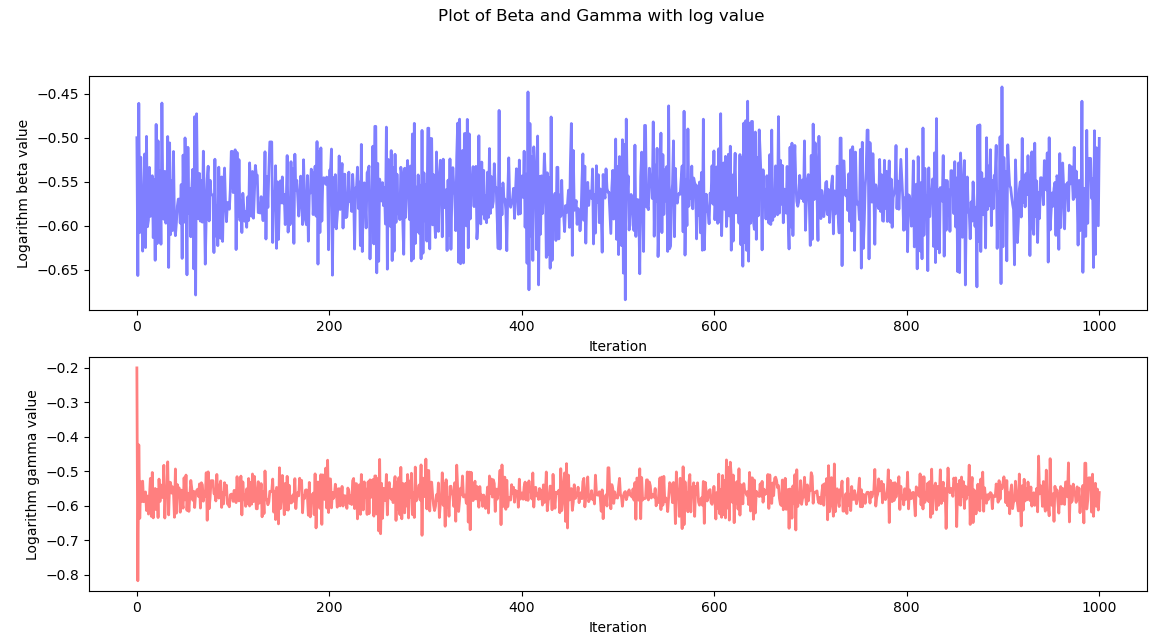
\includegraphics[scale=0.3]{Images/graph3.png}
\end{center}
\end{figure}

\end{enumerate}
\section{Bài toán 4}
\subsection{Thiết lập chương trình}\\
Tiến hành đưa dữ liệu từ github về máy với các số liệu SIR được cung cấp. Sử dụng thư viện {\tt pandas} của python với START\_DATE là ngày 22/1/2020
   	 \begin{mdframed}[hidealllines=true,backgroundcolor=magenta!10]
	 \begin{alltt}
def loadData(type, country):
    url = 'https://raw.githubusercontent.com/CSSEGISandData/COVID-19/master/csse_covid_19_data/csse_covid_19_time_series/time_series_covid19_'
    contentFile = requests.get(url + str(type) + '_global.csv').content
    df = pd.read_csv(io.StringIO(contentFile.decode('utf-8')))
    country_df = df[df['Country/Region'] == country]
    return country_df.loc[START_DATE:]
	 \end{alltt}
	 \end{mdframed}
Sau đó ta tiến hành xử lí và tính toán số liệu giá trị trung bình của $R_{0}$ từ công thức trong bài tập lớn.

\subsection{Phân tích kết quả}
\begin{enumerate}
    \item Chính sách:
    \begin{itemize}
        \item Phong tỏa Hồ Bắc: Vào ngày 23 tháng 1 năm 2020, chính quyền trung ương của Cộng hòa Nhân dân Trung Hoa áp đặt phong tỏa ở Vũ Hán, Hồ Bắc trong nỗ lực cách ly tâm chấn của dịch virus corona 2019–20 (2019-nCoV) để ngăn chặn dịch bệnh. Vào cuối ngày 24 tháng 1, tổng cộng có 12 đơn vị hành chính khác ở Hồ Bắc, từ cấp huyện đến cấp địa khu, bao gồm Hoàng Thạch, Kinh Châu, Nghi Xương, Hiếu Cảm, Kinh Môn, Tùy Châu, Hàm Ninh, Tiềm Giang, Tiên Đào, Thập Yển và Thiên Môn, bị hạn chế đi lạ
    \end{itemize}
    \item Phân tích:\\
Ta khảo sát trong khoảng thời gian trước khi tỉnh Hồ Bắc ban bố chính sách hạn chế di chuyển ngày là 22/1 đến ngày 23/7. Dựa vào số liệu được lấy từ trang \url{https://github.com/CSSEGISandData/COVID-19/tree/master/archived_data/archived_time_series}\\
ta ước lượng giá trị của hệ sổ $R_{0}$:
   	 \begin{mdframed}[hidealllines=true,backgroundcolor=magenta!10]
	 \begin{alltt}
Date:  1/22/20 ->R0:  7.657696161111439e-207
Date:  1/23/20 ->R0:  0.0
Date:  1/24/20 ->R0:  0.0
Date:  1/25/20 ->R0:  0.0
Date:  1/26/20 ->R0:  0.0
Date:  1/27/20 ->R0:  0.0
	 \end{alltt}
	 \end{mdframed}
    Với hệ số $R_{0}$ trước khi cách li là xấp xỉ bằng 0, và ở những ngày sau đó đã giảm xuống rất nhỏ dần dần về 0.
    Từ đây ta thấy với chính sách hạn chế di chuyển được ban hành như là giới hạn 7 ngày, đóng cửa các đường cao tốc, đang làm giảm việc tiếp xúc giữa mọi người, khiến cho việc lây lan dịch bệnh giảm xuống, tác động tương tự đến hệ số $R_{0}$.
\end{enumerate}
\section{Kết luận}
Trong báo cáo này chúng tôi đã trình bày tóm lược về việc sử dụng Python để giải một số bài toán về mô hình SIR và xử lý số liệu ở mức độ thống kê mô tả. Qua đó, giúp hiểu rõ được ý nghĩa của các mô hình dự báo, ứng dụng nó và cũng thông qua đó bước đầu nắm được việc sử dụng Python trong tình toán và phân tích dữ liệu.
%%%%%%%%%%%%%%%%%%%%%%%%%%%%%%%%%
\newpage
\addcontentsline{toc}{section}{Tài liệu}
\begin{thebibliography}{99999}
\bibitem[Dal]{Dal}{Dalgaard, P.} {\em Introductory Statistics with R.}  Springer 2008.

\bibitem[K-Z]{K-Z}{Kenett, R. S. and Zacks, S.}
{\em Modern Industrial Statistics: with applications in R, MINITAB and JMP,} 2nd ed.,  John Wiley and Sons, 2014.

\bibitem[Ker]{Ker}{Kerns, G. J.}
{\em Introduction to Probability and Statistics Using R,} 2nd ed., CRC 2015.
\bibitem[JKG20]{JKG20} T. Wu Joseph, Leung Kathy, and Leung Gabriel. “Nowcasting and forecasting the
potential domestic and international spread of the 2019-nCoV outbreak originating
in Wuhan, China: a modelling study”. In: 395 (2020).
\bibitem[LM05]{LM05} S. T. Ho Lam and A. Suchard Marc. Simple MCMC under SIR. 2005. \url{https://cran.r-project.org/web/packages/MultiBD/vignettes/SIR-MCMC.pdf.}
\end{thebibliography}
\end{document}